% section: 式の構造を使う解法

\section{式の構造を使う}\label{節：特殊性質型}

次の3つの\bookterm{recurrence}{漸化式}を見てほしい.
\[
  a_{n+1}=a_n^2,
  \quad
  a_{n+1}=a_n^2-1,
  \quad
  a_{n+1}=a_n^2-2
\]
1つ目は,更新するたびに指数が2倍になる.
繰り返し代入すれば
\[
  a_n=a_1^{2^{n-1}}
\]
と分かる.$a_1>0$なら\bookterm{logarithm}{対数}で\bookterm{geometric}{等比数列}にもできる.
$a_1\le0$では実数の対数を最初から取れないが,元の更新は定義される.

2つ目は$-1$が対数の利用を妨げる.\bookterm{fixed}{不動点}は
\[
  \alpha=\alpha^2-1
  \quad\Longleftrightarrow\quad
  \alpha=\frac{1\pm\sqrt5}{2}
\]
であり,初項をこれに選べば定数解となる(\sectionref{節：初項依存型}).
ただし,$b_n=a_n-\alpha$と置いても,
\[
  b_{n+1}=b_n^2+2\alpha b_n
\]
と二次の項が残り,\bookterm{linear}{線形}にはならない.
ここまでの手法では閉じた\bookterm{general}{一般項}を得られないが,他の解法まで否定したわけではない.\footnote{ここでいう閉じた式の意味と,「解く」ことの範囲については\sectionref{節：漸化式の分類}で考える.}

3つ目の$-2$は,ある恒等式にちょうど合う.
基本型への変形が見つからなくても,\textbf{式に固有の構造}から解法が開けることがある.
この節では,その一致を見ていこう.

\subsection{対称式を使う}\label{節：基本対称式型}
先ほどの\bookterm{recurrence}{漸化式}を考える.
\[
  a_1=3, \quad a_{n+1}=a_n^2-2
\]
邪魔な$-2$を消すには,二乗の展開から$2$を生み出したい.そこで,
\[
  (a+b)^2=a^2+2ab+b^2
\]
の$2ab$に注目する.$ab=1$なら,ここからちょうど$2$が生まれる.
    そこで積が$1$になる二数として,$a=\alpha,b=\dfrac{1}{\alpha}\ (\alpha\ne0)$と選ぶ.
\[
  \left(\alpha+\frac{1}{\alpha}\right)^2=\alpha^2+2+\frac{1}{\alpha^2}
\]
から,\textbf{二乗して2を引くと,二つのべきの指数が2倍になる}.
第$n$項の指数は$2^{n-1}$.あとは初項に合う$\alpha$を選ぶ.

\noindent \bookblocklink{example-symmetric-1}{problem}{answer}{【問題】}\par\nobreak
\begin{smallquote}
  次の\bookterm{recurrence}{漸化式}で定義される\bookterm{sequence}{数列}の\bookterm{general}{一般項}を求めよ.
  \[
    a_1=3, \quad a_{n+1}=a_n^2-2
  \]
\end{smallquote}
\bookblocklink{example-symmetric-1}{answer}{problem}{【解答】}
  \begin{smallquote}
  \bookterm{general}{一般項}が
    \[
      b_n=\alpha^{2^{n-1}}+\alpha^{-2^{n-1}}
    \]
    で表される\bookterm{sequence}{数列}$b_n$を考える.
    \begin{align*}
      b_{n+1}&=\alpha^{2^{n}}+\alpha^{-2^{n}}\\
      &=\left(\alpha^{2^{n-1}}+\alpha^{-2^{n-1}}\right)^2-2\\
      &=b_n^2-2
    \end{align*}
    と更新が一致する.初項を合わせると,
    \begin{align*}
      &\alpha+\alpha^{-1}=3\\
      &\alpha^2-3\alpha+1=0\\
      &\therefore \quad \alpha=\frac{3\pm \sqrt{5}}{2}
    \end{align*}
    二つの根は互いに逆数で,同じ$b_n$を与える.初項と更新の一致から,
    \[
      a_n=\left(\frac{3+ \sqrt{5}}{2}\right)^{2^{n-1}}+\left(\frac{3- \sqrt{5}}{2}\right)^{2^{n-1}}
    \]
  \end{smallquote}

ここで,定数を $-2$ から $-1$ に変えてみよう.
\[
  a_{n+1}=a_n^2-1
\]
同じ置換では,
\begin{align*}
  a_n^2-1
    &=\left(u+u^{-1}\right)^2-1\\
    &=u^2+u^{-2}+1,
\end{align*}
と余分な1が残り,同じ形で二乗を繰り返すことができない.
係数が近いだけでは同じ方法を使えず,恒等式との一致が必要なのである.

同じ考え方は,三次式にも現れる.
\[
  \left(\alpha+\frac{1}{\alpha}\right)^3
  -3\left(\alpha+\frac{1}{\alpha}\right)
  =\alpha^3+\frac{1}{\alpha^3}
\]
対称な組み合わせを保ったまま,指数を3倍できる.

和を取るか差を取るかで,打ち消せる項の符号も変わる.
差の三乗を展開すれば,
\[
  \left(\alpha-\frac{1}{\alpha}\right)^3
  +3\left(\alpha-\frac{1}{\alpha}\right)
  =\alpha^3-\frac{1}{\alpha^3}
\]
となる.指数$3^{n-1}$の候補を例題で確かめよう.

\noindent\bookblocklink{example-symmetric-2}{problem}{answer}{【問題】}\par\nobreak
\begin{smallquote}
  $\displaystyle a_1=\frac{8}{3},\quad a_{n+1}=a_n^3+3a_n$
\end{smallquote}
\bookblocklink{example-symmetric-2}{answer}{problem}{【解答】}
\begin{smallquote}
  \bookterm{general}{一般項}が
    \[
      b_n=\alpha^{3^{n-1}}-\alpha^{-3^{n-1}}
    \]
    で表される\bookterm{sequence}{数列}$b_n$を考える.
    \begin{align*}
      b_{n+1}&=\alpha^{3^{n}}-\alpha^{-3^{n}}\\
      &=b_n^3+3b_n
    \end{align*}
    と更新が一致する.初項を合わせると,
    \begin{align*}
      &\alpha-\alpha^{-1}=\frac{8}{3}\\
      &3\alpha^2-8\alpha-3=0\\
      &\therefore \quad \alpha=3,\,-\frac13
    \end{align*}
    $3^{n-1}$は奇数なので,どちらを選んでも$b_n$は同じ値になる.
    初項と更新の一致から,$\alpha=3$を選べば,
    \[
      a_n=3^{3^{n-1}}-3^{-3^{n-1}}
    \]
\end{smallquote}

\subsection{三角関数型}\label{節：三角関数型}
  \subsubsection{角度に置き換える}\label{節：解法}
    次の\bookterm{recurrence}{漸化式}を考える.
    \[
      a_1=\frac{\sqrt{3}}{2},\quad a_{n+1}=2a_n^2-1
    \]

    $t_n=2a_n$なら$t_{n+1}=t_n^2-2$と前節につながる.
    別の入口として,\bookterm{trigonometric}{三角関数}の公式$\cos2x=2\cos^2x-1$に注目する.
    右辺の二乗と$-1$が,与えられた更新と一致している.
    項を余弦の値として表せれば,次の項は角度を2倍した余弦になる.
    初項も
    \[
      a_1=\cos\frac{\pi}{6}
    \]
    と書ける.そこで $a_n=\cos\theta_n$ と置くと,
    \[
      \theta_1=\frac{\pi}{6},
      \quad
      \theta_{n+1}=2\theta_n
    \]
    と選べばよい.$\cos$の値から角度は一意に決まらないので,倍角は更新を満たす候補を作るための選び方である.
    候補は
    \[
      a_n=\cos\left(2^{n-1}\frac{\pi}{6}\right)
    \]
    である.

    $n=1$で初項に一致する.$n$で成り立つなら,
    \begin{align*}
      a_{n+1}
        &=2a_n^2-1\\
        &=2\cos^2\left(2^{n-1}\frac{\pi}{6}\right)-1\\
        &=\cos\left(2^n\frac{\pi}{6}\right)
    \end{align*}
    となり,帰納法で示される.二次式の更新を,角度の2倍へ翻訳した.

  \subsubsection{倍角と回転}\label{節：倍角を回転として見る}
    単位円上で,正の$x$軸からの角が$\theta$の点を
    \[
      P(\theta)=(\cos\theta,\sin\theta)
    \]
    とする.原点$O$のまわりにさらに$\theta$回すと$P(2\theta)$へ移る.
    倍角は,\textbf{現在の角度だけ,もう一度回す操作}である.

    \begin{center}
      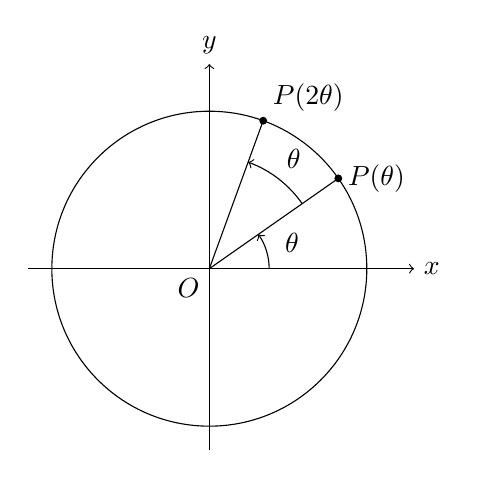
\begin{tikzpicture}[scale=2]
        \draw[->] (-1.15,0) -- (1.3,0) node[right] {$x$};
        \draw[->] (0,-1.15) -- (0,1.3) node[above] {$y$};
        \draw (0,0) circle (1);
        \node[below left] at (0,0) {$O$};
        \draw (0,0) -- (35:1);
        \draw (0,0) -- (70:1);
        \fill (35:1) circle (0.025) node[right] {$P(\theta)$};
        \fill (70:1) circle (0.025) node[above right] {$P(2\theta)$};
        \draw[->] (0.38,0) arc (0:35:0.38);
        \node at (17.5:0.55) {$\theta$};
        \draw[->] (35:0.72) arc (35:70:0.72);
        \node at (52.5:0.88) {$\theta$};
      \end{tikzpicture}
      \BookFigureCaption{単位円における角度の倍化}
    \end{center}

    先ほどの\bookterm{sequence}{数列}では,$a_n$は点$P(\theta_n)$の横座標である.
    回転後の横座標が
    \[
      \cos(2\theta_n)=2\cos^2\theta_n-1=2a_n^2-1
    \]
    となり,更新を満たす.初めの角度は
    \[
      \frac{\pi}{6}\ \longrightarrow\ \frac{\pi}{3}
      \ \longrightarrow\ \frac{2\pi}{3}
      \ \longrightarrow\ \frac{4\pi}{3}
    \]
    と変わり,横座標は
    \[
      \frac{\sqrt{3}}{2}\ \longrightarrow\ \frac12
      \ \longrightarrow\ -\frac12
      \ \longrightarrow\ -\frac12
    \]
    と変わる.最後の二点は異なるが横座標は同じであり,\bookterm{sequence}{数列}の値だけでは点の動きを捉えきれない.

    一定角の回転なら$\theta_{n+1}=\theta_n+\phi$だが,倍角では回す角度が毎回変わる.
    点の角度は$2\pi$ごとに読み替えてよい.$P(\theta)$と$P(\theta+\pi)$は倍角で同じ点へ移るため,円周全体の写像としても一定角の回転とは異なる.

    \,\sectionref{節：極形式と複素平面}の見方を使えば,この操作はさらに短く書ける.
    \[
      z_n=\cos\theta_n+i\sin\theta_n
    \]
    と置くと,\bookterm{de-moivre}{ド・モアブルの定理}より
    \[
      z_{n+1}=z_n^2,\qquad z_n=z_1^{\,2^{n-1}}
    \]
    となる.絶対値1の$z_n$を自身に掛け,角度をもう一度加えた.$a_n$はその実部である.

    \subsubsection{正接と傾き}\label{節：正接では直線の傾きを記録する}
    今度は
    \[
      a_1=\tan\frac{\pi}{12}=2-\sqrt{3},
      \quad
      a_{n+1}=\frac{2a_n}{1-a_n^2}
    \]
    を考える.右辺は$\tan$の倍角公式そのものである.したがって,
    \[
      a_n=\tan\left(2^{n-1}\frac{\pi}{12}\right)
    \]
    と予想できる.

    初項に一致し,帰納法の段階では
    \begin{align*}
      a_{n+1}
        &=\frac{2a_n}{1-a_n^2}\\
        &=\cfrac{2\tan\left(2^{n-1}\cfrac{\pi}{12}\right)}
                {1-\tan^2\left(2^{n-1}\cfrac{\pi}{12}\right)}\\
        &=\tan\left(2^n\frac{\pi}{12}\right)
    \end{align*}
    となる.分母が0にならないことは,角度から確かめる.

    $a_n=\tan\theta_n$は,原点と$P(\theta_n)$を通る直線の傾きである.
    倍角の動きを,今度は横座標でなく傾きで記録する.
    直線の向きは$\pi$ごとに同じになるが,縦向きでは傾きが定義できない.
    $a_n=\pm1$では$\cos(2\theta_n)=0$となり,この縦向きが分母$1-a_n^2=0$に対応する.
    なお,この例の角度は,$n\geq2$では
    \[
      \theta_n=\frac{2^{n-2}\pi}{6}
    \]
    である.$\displaystyle \theta_n=\frac{\pi}{2}+k\pi$となるには$2^{n-2}=3+6k$が必要だが,
    2の累乗は3の倍数でないので不可能である.初項でも傾きは定義できるため,全項が定義される.

  \subsubsection{角度の整数倍}\label{節：整数倍の公式へ}
    両例の方針は,
    \[
      a_n=\varphi(\theta_n),
      \quad
      \varphi(m\theta)=F_m(\varphi(\theta))
    \]
    を満たす関数と整数倍公式を探し,角度の更新を解くことである.

    また,ここで現れた多項式
    \[
      2x^2-1,
      \quad
      4x^3-3x
    \]
    も同じ族に属する.\bookterm{chebyshev}{チェビシェフ多項式}$T_m(x)$を
    \[
      T_m(\cos\theta)=\cos(m\theta)
    \]
    で定義すれば,
    \[
      T_0(x)=1,  T_1(x)=x,
    \]
    \[
      T_{m+1}(x)=2xT_m(x)-T_{m-1}(x)
    \]
    となる.例えば $T_2(x)=2x^2-1$ である.
    $T$の添字は角度の倍率なので,$\cos$の例は
    \[
      a_{n+1}=T_2(a_n),
      \quad
      a_n=T_{2^{n-1}}(a_1)
    \]
    と書ける.一回の更新では
    \[
      T_2(T_m(\cos\theta))=T_{2m}(\cos\theta)
    \]
    となり,添字は$2,4,8,\ldots$と進む.
    付録の\bookterm{chebyshev}{チェビシェフ多項式}では,この合成を一般の整数倍へ広げる.

\subsection{ニュートン法}\label{節：ニュートン法型}

方程式の解へ近づく更新を,接線の傾き$f'(a)$から設計する.\footnote{微分が未習なら,接線と$x$軸の交点から次の近似値を作る図形的な発想と,得られた\bookterm{recurrence}{漸化式}の変形を先に読んでよい.}
点$a$の近くでは,
\[
  f(a+h) \approx f(a)+f'(a)h
\]
と近似できる.方程式
\[
  f(x)=x^2-2=0
\]
の正の解を求めよう.正の近似値$a_n$での接線は,傾き$2a_n$より,
\[
  y=f(a_n)+2a_n(x-a_n)
\]
である.\,$y=0$ と置いて $x$ 軸との交点を求めると,
\begin{align*}
  a_{n+1}
    &=a_n-\frac{f(a_n)}{f'(a_n)}\\
    &=a_n-\frac{a_n^2-2}{2a_n}\\
    &=\frac{a_n^2+2}{2a_n}
\end{align*}
を得る.これが\bookterm{newton}{ニュートン法}の\bookterm{recurrence}{漸化式}である.
$a_1>0$から各項も正となり,分母は0にならない.
  \BookFigNewton

例えば $a_1=2$ とすると,
\[
  a_2=\frac{3}{2},
  \quad
  a_3=\frac{17}{12},
  \quad
  a_4=\frac{577}{408}
\]
となり,これらは $\sqrt{2}$ に急速に近づく.この速さは,誤差を
$e_n=a_n-\sqrt{2}$ と置くと見える.
\begin{align*}
  e_{n+1}
    &=\frac{a_n^2+2}{2a_n}-\sqrt{2}\\
    &=\frac{(a_n-\sqrt{2})^2}{2a_n}\\
    &=\frac{e_n^2}{2a_n}
\end{align*}
誤差が小さくなると,分母は$2\sqrt2$に近づき,誤差は二乗に応じて減る.
\bookterm{general}{一般項}を求めるには,残る分母$a_n$を消したい.
$a_n-\sqrt2$と$a_n+\sqrt2$を並べると,
\BookMathLayout{
\[
\begin{aligned}
a_{n+1}-\sqrt2&=\frac{(a_n-\sqrt2)^2}{2a_n},\\
a_{n+1}+\sqrt2&=\frac{(a_n+\sqrt2)^2}{2a_n}
\end{aligned}
\]
}{
\[
\begin{aligned}
a_{n+1}-\sqrt2&=\frac{(a_n-\sqrt2)^2}{2a_n},\\
a_{n+1}+\sqrt2&=\frac{(a_n+\sqrt2)^2}{2a_n}
\end{aligned}
\]
}
となる.両辺の比を取ることで$2a_n$が消え,
\[
  \frac{a_{n+1}-\sqrt{2}}{a_{n+1}+\sqrt{2}}
  =\left(\frac{a_n-\sqrt{2}}{a_n+\sqrt{2}}\right)^{2}
\]
となる.そこで
\[
  b_n=\frac{a_n-\sqrt{2}}{a_n+\sqrt{2}}
\]
と置けば,$b_{n+1}=b_n^2$と\bookterm{logarithm}{対数}型(\sectionref{節：対数型})へ戻る.
\textbf{そのまま二乗されるのは誤差$e_n$ではなく,比$b_n$である.}

\,$a_1=2$のとき,\,$b_1=\dfrac{2-\sqrt2}{2+\sqrt2}=3-2\sqrt2=\dfrac1{3+2\sqrt2}$であるから,\,$u=3+2\sqrt2$とおくと$b_n=u^{-2^{n-1}}$である.これを$b_n=\dfrac{a_n-\sqrt2}{a_n+\sqrt2}$について$a_n$で解けば,
\[
  a_n=\sqrt{2}\,\frac{u^{2^{n-1}}+1}{u^{2^{n-1}}-1},\qquad u=3+2\sqrt2
\]
という閉じた式が得られる.
$u>1$なので,$u^{-2^{n-1}}$は$0$に近づき,$a_n$は$\sqrt2$に近づくことも分かる.

この閉じた式は$f(x)=x^2-2$に固有の変形から得たものである.
一般の\bookterm{newton}{ニュートン法}でも得られるとは限らないが,収束先や誤差は調べられる.
\sectionref*{節：差分から始まる離散的な微積分}では,更新の設計を収束,\bookterm{fixed}{不動点},誤差評価,微分方程式へ広げる.

\subsection{初項による違い}\label{節：初項依存型}

式の形に加えて,初項の選び方も解法を左右する.
\[
  a_1=c,
  \quad
  a_{n+1}=\frac{a_n^2-1}{2}
\]
初項を記号 $c$ のままにすると,
\begin{align*}
  a_2&=\frac{c^2-1}{2},\\
  a_3&=\frac{c^4-2c^2-3}{8},\\
  a_4&=\frac{c^8-4c^6-2c^4+12c^2-55}{128}
\end{align*}
一般に$a_n$は$c$の次数$2^{n-1}$の多項式となり,固定された簡単な表現が見えにくい.

特に $c=2$ と固定すると,
\[
  a_1=2,
  \quad
  a_2=\frac{3}{2},
  \quad
  a_3=\frac{5}{8},
  \quad
  a_4=-\frac{39}{128}
\]
となる.倍角や対称式の恒等式,接線近似はそのまま使えない.
  図では$f(x)=\dfrac{x^2-1}{2}$とし,$a_1=2$から曲線$y=f(x)$へ縦に進み,直線$y=x$へ横に進む.
  縦の移動で次の値を計算し,横の移動でそれを次の入力にする.
  初項を変えれば,同じ更新でも別の軌道をたどる.
  \BookFigCobweb

$c=2$で簡単な表現が見えなくても,他の初項まで同じとは限らない.
例えば,
\[
  c=1+\sqrt{2},
  \quad
  c=1-\sqrt{2}
\]
なら定数\bookterm{sequence}{数列}$a_n=c$となる.
一般の$c$では閉じた\bookterm{general}{一般項}が見つからなくても,
\[
  a_n=f^{\,\circ(n-1)}(c),
  \quad
  f(x)=\frac{x^2-1}{2}
\]
と書くことはできる.\footnote{$f^{\,\circ m}$は$f$を$m$回合成することを表し,$f^{\,\circ0}(c)=c$とする.関数の値の$m$乗とは異なる.}
これは更新の略記で,計算を済ませた式ではない.軌道,\bookterm{limit}{極限},近似を調べることもできる.
付録では\bookterm{matrix}{行列}や\bookterm{generating}{母関数}へ見方を広げる.

基本対称式型も,初項次第では直接分かる.
\[
  a_1=-1,\quad a_{n+1}=a_n^2-2
\]
なら$a_n=-1$となる.定数解は\bookterm{fixed}{不動点}の式
\[
  \alpha=\alpha^2-2
\]
の解$\alpha=-1,2$を初項に選べば得られる.

定数解$a_n=-1$も,\sectionref{節：基本対称式型}の$\alpha+\alpha^{-1}=a_1$による表示に含まれる.
その計算を複素数へ広げよう.\footnote{$\alpha^2-a_1\alpha+1=0$には複素数の範囲で必ず非零の解がある.$|a_1|<2$では$\alpha$が実数にならないため,実数の$\alpha$だけを使った先の例から一歩広げている.}
特に$-2\le a_1\le2$なら,$a_1=2\cos\theta$と書けるので,
$\alpha=e^{i\theta}$と選ぶと
\[
  a_n=\alpha^{2^{n-1}}+\alpha^{-2^{n-1}}=2\cos(2^{n-1}\theta)
\]
という\bookterm{trigonometric}{三角関数}の形になる.

$a_1=-1$では$\theta=\dfrac{2\pi}{3}$.倍角を$2\pi$ごとに読み替えると,$\dfrac{2\pi}{3}$と$\dfrac{4\pi}{3}$を行き来する.
どちらも余弦が$-\dfrac{1}{2}$なので$a_n=-1$となる.角度の動きを横座標に移すと,定数解になった.

\subsection{変わらない量を使う}\label{節：不変量から線形の関係}
  \sectionref*{節：基本対称式型}の恒等式に続き,\textbf{更新しても変わらない関係}を探す.
  それを使い,\sectionref*{節：隣接3項間漸化式型}へ帰着させる.

  \subsubsection{例題：数項から候補を作る}
  \[
    a_1=a_2=1,\qquad
    a_{n+2}=\frac{a_{n+1}^2+1}{a_n}\quad(n\ge1)
  \]
  を考える.初めの数項は$1,1,2,5,13,\ldots$である.
  正の二項から次の項も正になるので,すべての分母は非零である.
  $a_{n+2}=3a_{n+1}-a_n$と予想できるが,証明が要る.
  $x=a_n,y=a_{n+1},z=a_{n+2}$とすれば$xz=y^2+1$で,$x,z$が対称に現れる.
  $x+z=Ky$を目標にすると,係数の候補は
  \[
    K=\frac{x+z}{y}=\frac{x^2+y^2+1}{xy}
  \]
  となる.\textbf{目標から,一定であってほしい量を作った.}

  \bookstep{変わらないことを示す}
  作った量を
  \BookMathLayout{\[
    I_n=\frac{a_n^2+a_{n+1}^2+1}{a_na_{n+1}}
  \]}{\[
    \begin{aligned}
      I_n=\frac{a_n^2+a_{n+1}^2+1}{a_na_{n+1}}
    \end{aligned}
  \]}
  とする.$xz=y^2+1$より,
  \[
    \begin{aligned}
      \frac{x^2+y^2+1}{xy}&=\frac{x+z}{y},\\
      \frac{y^2+z^2+1}{yz}&=\frac{x+z}{y}
    \end{aligned}
  \]
  なので$I_{n+1}=I_n$である.
  $I_1=3$だから,すべての$n$について
  \[
    a_n+a_{n+2}=3a_{n+1}
  \]
  を得る.初めの二項を保ったまま\bookterm{linear}{線形}の\bookterm{recurrence}{漸化式}へ帰着できた.

  \bookstep{一般項へ戻す}
  $\alpha=\frac{3+\sqrt5}{2}$, $\beta=\frac{3-\sqrt5}{2}$とすると,
  \bookterm{characteristic}{特性方程式}$x^2-3x+1=0$から
  \[
    a_n=\frac{\alpha^{n-1}+\beta^{n-1}}2
       -\frac{\alpha^{n-1}-\beta^{n-1}}{2\sqrt5}
  \]
  を得る.初めの二項はともに1で,線形の更新の一意性から元の数列に一致する.
  また,$a_{n+2}=3a_{n+1}-a_n$から整数性も帰納的に分かる.

  \subsubsection{保存と線形化}
  更新の前後で値が変わらない量を\textbf{\bookterm{invariant}{不変量}}という.
  この例題では,保存される量から足し算と定数倍の\bookterm{linear}{線形}の関係を取り出した.\footnote{この\bookterm{linear}{線形}の式と元の式が全く同じ条件を表すと無条件に主張したわけではなく,
  元の数列について保存から導いた関係である.}

  \begin{bookpoint}
    \textbf{\bookterm{invariant}{不変量}の使い方}\par
    初期値で保存量の値を決め,元の更新と合わせて解きやすい関係を取り出す.
    保存量の存在だけで\bookterm{general}{一般項}が求まるとは限らない.
  \end{bookpoint}
  初期値を変えたときの係数は\bookproblemref{practice-connections}{2}{接続演習問2},
  整数方程式を保つ更新は\bookproblemref{practice-entrance}{9}{発展問9}へ.
  付録の\sectionref*{節：演習の操作を別の表現で見直す}でも発展問9を扱う.

\subsection{非線形の周期性}\label{節：非線形の周期性}
  \sectionref*{節：初項依存型}の定数解に続き,二項の組が戻ることで周期を示す.
  \bookterm{general}{一般項}は先に求めなくてよい.

  \bookstep{例：二項の組が戻る}
  $a_{n+2}=\dfrac{1+a_{n+1}}{a_n}$で初めの二項をともに$1$にすると,
  $1,1,2,3,2,1,1,\ldots$となる.
  第6,7項が初めの二項に戻るので,その先も繰り返す.正の$x,y$へ広げよう.

  \bookstep{一般の初期値で確かめる}
  \[
    \begin{aligned}
      a_1&=x>0,\qquad a_2=y>0,\\
      a_{n+2}&=\frac{1+a_{n+1}}{a_n}\quad(n\ge1)
    \end{aligned}
  \]
  とする.正の二項から次も正になるため,すべての項が定義される.

  \bookstep{最初の二項への復帰}
  \BookMathLayout{\[
    a_3=\frac{1+y}{x},\qquad
    a_4=\frac{1+x+y}{xy},\qquad
    a_5=\frac{1+x}{y}
  \]}{\[
    \begin{aligned}
      a_3&=\frac{1+y}{x},\\
      a_4&=\frac{1+x+y}{xy},\\
      a_5&=\frac{1+x}{y}
    \end{aligned}
  \]}
  となる.$a_5$では
  \[
    a_5=\frac{xy+1+x+y}{y(1+y)}=\frac{1+x}{y}
  \]
  と因数分解した.さらに
  \[
    a_6=\frac{1+a_5}{a_4}=x,\qquad
    a_7=\frac{1+a_6}{a_5}=y
  \]
  と二項の組が戻り,その先も同じ更新で決まる.従って,
  \[
    a_{n+5}=a_n\qquad(n\ge1)
  \]
  である.

  \bookstep{周期と最小周期}
  定\bookterm{sequence}{数列}になる$x=y=\dfrac{1+\sqrt5}{2}$では最小周期は1,ほかは5である.
  定数解の条件は$x=y=t>0$, $t^2=t+1$から得る.
  最小周期は5の約数である.そうでなければ,5を最小周期で割った正の余りも周期となり,最小性に反する.

  \begin{bookpoint}
    \textbf{周期を証明する条件}\par
    二項で更新が決まるなら,二項の組の復帰を示す.
    初項からの周期,途中からの周期,符号だけの振動は区別する.
  \end{bookpoint}
  \sectionref*{節：ガウス型}の有限状態,\sectionref*{節：虚数解型隣接3項間漸化式}の回転とは別の周期の仕組みである.
  初項の例外は\bookproblemref{practice-connections}{5}{接続演習問5}で確かめよう.

